\newpage
\section{Project Implementation}
\subsection{Deliverables}
The Big Data Auto-Tuning tool is a solution to finding optimum configuration for big data applications, helping developers with little or no knowledge of the underlying big data technologies automatically improving their application’s performance.\\
The implementation of the tool has two main parts, which consist of the following deliverables:
\begin{itemize}
\item -	Provide a development environment in the Eclipse IDE, where developers can explore configuration optimisation and the performance of their applications.
	\begin{itemize}
	\item Allow selection of configuration parameters of corresponding big data technology for optimisation
    \item Allow specification of parameter values, ranges and intervals to experiment upon
    \item Extend BO4CO tool to support broader types of input: boolean, categorical, ranges and intervals.
    \item Allow configuration of experiment set-up, eg: test application to run, numbers of iterations and experiment time
    \item Allow setting of connections to remote Jenkins server, remote testbed and monitoring services 
	\end{itemize}
\item -	Fully integrate the development environment to trigger configuration optimisation on remote automation server and run tests on remote testbed.
	\begin{itemize}
	\item Integrate Eclipse and Jenkins for triggering parameterised builds with configuration files remotely
    \item Integrate Jenkins automation server and MATLAB-based BO4CO tool to start experiment
	\item Integrate BO4CO tool and remote Storm testbed to deploy tests with different configuration parameters and retrieve performance metrics
    \item Integrate Eclipse and Jenkins to retrieve and display BO4CO configuration results
	\end{itemize}
\end{itemize}

\newpage
\subsection{Big Data Auto-tuning Tool Design}
The Big Data Auto-tuning Tool builds upon the structure of the Configuration Optimization tool, detailed in Figure \ref{fig:cotool}. The tool adds two main parts, a user interface on the Eclipse integrated development environment, and a Jenkins server instance that automates execution of the Configuration Optimisation tool.
\begin{figure}[h]
\centering
\caption{Big Data Auto-tuning Tool.}
\label{fig:tooldesign}
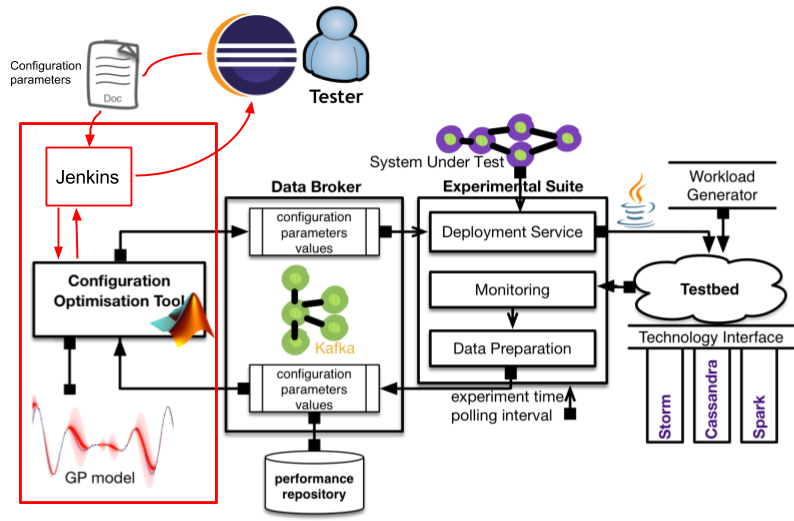
\includegraphics[width=\textwidth]{images/tooldesign.png}
\end{figure}
As seen in Figure \ref{fig:tooldesign}, the developer selects configuration parameters to optimise via the user friendly interface on the Eclipse IDE. The experiment configuration file is generated according to the selections, and sent to the remote Jenkins CI server as it triggers the experiment to run. Jenkins executes the Configuration Optimisation tool, and monitors the status of the experiment. When the CO tool terminates, Jenkins retrieves the results and the optimised configuration. The developer can access the results conveniently from the Eclipse IDE.\\
The Big Data Auto-tuning Tool provides a fully integrated solution in the development environment to performance test and tune big data applications, in line with the DevOps principles of frequent testing in deployment environment. In comparison to the existing approach to directly work with the Configuration Optimisation tool, the developer can now run optimisation and view results without leaving the IDE. The developer no longer manually creates an experiment configuration file for the tool. The GUI lists the configuration parameters available for selection for the corresponding big data framework, provided helpful descriptions to aid non-expert developers. It simplifies the process for the developer, without requiring that he understands the format of the CO tool's experiment configuration file. It also eliminates human error in creating the file and guarantees no parsing problem when it is executed. The Big Data Auto-tuning Tool allows the use of a remote Jenkins server to execute experiments. The developer no longer has to have terminal access to the machine hosting the CO tool to run and monitor experiments. Jenkins remotely runs and retrieves results, leaving the developer free on his machine. The results are retrieved and clearly displayed, again requiring no access outside of the IDE. 

\newpage
\subsection{Project Management and Risks}
\subsubsection{Original Timetable}
\begin{center}
\begin{tabular}{|c|c|}
\hline
Month & Milestone\\
\hline
March '17 & Investigate and implement the integration of Eclipse and Jenkins\\
\hline
April '17 & Create UI in the Eclipse IDE to select configuration parameters\\
 & Complete UI in the Eclipse IDE to collect experiment settings\\
\hline
May '17 & Set up Jenkins automation for execution of BO4CO with integration to\\
&  testbed. Retrieve results to Eclipse and display optimal configuration.\\
\hline
\end{tabular}
\end{center}

\subsubsection{Risks}
There are significant risks in implementing the Big Data Auto-tuning tool, due to the complexity of coordinating the numerous components involved. The integration of all parts is the main challenge of this project, and the reward is that developers using the tool will have a smooth and integrated experience without the hassle of manually setting up each component to interface with each other. Some components reside on different remote servers and require connections to be established, and the components are built on different technologies and programming languages.\\
The integration between Eclipse and Jenkins was the first risk. The state of the art integration is provided by  the Hudson/Jenkins Mylyn Builds Connector \cite{mylyn}, which does not support triggering parameterised builds on the Jenkins server from Eclipse. Jenkins provides an API for triggering parameterised builds, but the specific requirements to include a file parameter was not documented \cite{pbuild}, although an example using cURL was given \cite{remoteapi}. It remained unclear what the general requirement was, and was unclear how to replicate the command in a Java / Apache-based HTTP client. As the configuration file parameter is crucial to this project, this was the first risk to tackle. A fall back option was also planned to parse an entire file into a String and trigger the parameterised build with a String parameter, which was a well-documented approach. \cite{pbuild}\\
The dependency of this project on core BO4CO code poses a big risk. It has to be assumed that BO4CO code provided was working as designed. The extension of BO4CO functionality to accept different input types to support categorical values in addition to integer values is also challenging because it requires changing the data type used internally, and the changes propaginate to the entire system that is tightly coupled.\\
The execution of experiments for configuration optimisation created a lot of dependencies on the big data frameworks installed on the testbed. The state of each of the following services each posed a risk to the successful integration of this project. If any of these services did not behave as they are designed to, or if there is any update that introduced incompatibilities, the project would be at risk of failing. 
\begin{itemize}
\item DICE Jenkins Continuous Integration service - for monitoring experiments
\item DICE Deployment Service - for deploying experiments
\item DICE Monitoring Platform - to monitor performance of experiments
\item Storm cluster - for executing experiments
\item Zookeeper cluster - for deploying experiments
\item Kafka cluster - for deploying experiments
\item Hadoop cluster - for executing experiments
\end{itemize}
The integration between Jenkins and the MATLAB-based BO4CO code is also a risk. Unlike projects in Java or those managed by Gradle, Ant and Maven, MATLAB projects are not supported by a Jenkins plugin. The execution will have to be controlled by executing scripts, which make the implementation dependent and susceptible to changes in the host platform. There is an unofficial guide on MATLAB continuous integration using Jenkins written for Linux users, but there is no support for developers on Windows machines.

\subsubsection{Project Time line}
The initial stages of the project proceeded as planned in the original timetable. However, as mentioned in the risks above, the execution of BO4CO proved to be problematic. The problems encountered are documented in the later sections on BO4CO and integration with Jenkins and the testbed.\\
These difficulties caused the completion of the project deliverables to be delayed into June. In the interest of delivering a fully integrated development environment as specified in the deliverables, time and effort was dedicated to fully integrating all services to support Storm big data framework. Validation for use with the Hadoop framework was not completed, although support for the Hadoop framework had been built in.
\begin{center}
\begin{tabular}{|c|c|}
\hline
Month & Progress\\
\hline
March '17 & \multirow{2}{*}{\parbox{12cm}{Integrate Eclipse and Jenkins for triggering parameterised builds with configuration files remotely.}}\\
&\\
\hline
April '17 & \multirow{4}{*}{\parbox{12cm}{Create UI to allow selection of configuration parameters. Allow specification of parameter values, ranges and intervals to experiment upon. Collection of experiment settings, connections to remote Jenkins server remote testbed and monitoring services.}}\\
&\\
&\\
&\\
\hline
May '17 & \multirow{1}{*}{\parbox{13cm}{Refine and complete Eclipse UI.}}\\
& \multirow{4}{*}{\parbox{12cm}{Integrate BO4CO tool and remote Storm testbed to deploy tests with different configuration parameters and retrieve performance metrics. Integrate Eclipse and Jenkins to retrieve and display BO4CO configuration results.}}\\
&\\
&\\
&\\
\hline
June '17 & \multirow{3}{*}{\parbox{12cm}{Integrate Jenkins automation server and MATLAB-based BO4CO tool to start experiment. Extend BO4CO tool to support broader types of input: boolean, categorical, ranges and intervals.}}\\
&\\
&\\
\hline
\end{tabular}
\end{center}